%%
% This is an Overleaf template for presentations
% using the TUM Corporate Desing https://www.tum.de/cd
%
% For further details on how to use the template, take a look at our
% GitLab repository and browse through our test documents
% https://gitlab.lrz.de/latex4ei/tum-templates.
%
% The tumbeamer class is based on the beamer class.
% If you need further customization please consult the beamer class guide
% https://ctan.org/pkg/beamer.
% Additional class options are passed down to the base class.
%
% If you encounter any bugs or undesired behaviour, please raise an issue
% in our GitLab repository
% https://gitlab.lrz.de/latex4ei/tum-templates/issues
% and provide a description and minimal working example of your problem.
%%

\documentclass{setbeamer}

\usepackage{tikz}
\usetikzlibrary{calc}
\usetikzlibrary{positioning}

\usepackage{marvosym}

% https://tex.stackexchange.com/questions/196794/how-can-you-create-a-vertical-timeline
% Style and colors adjusted for TUM-Theme
\usepackage{xcolor}
% maybe vline after {$bullet$} for visual clarity, but this produced seams. I couldn't get rid of them...
\newcommand\ytl[2]{
\parbox[b]{8em}{\hfill{\color{TUMExtTeal}\bfseries\sffamily #1}~$\cdots\cdots$~}\,\makebox[0pt][c]{$\bullet$}\quad \parbox[c]{4.5cm}{\vspace{7pt}\color{TUMGrayDark}\raggedright\sffamily #2\\[7pt]}\\[-3pt]}

\newcommand{\myline}[3][TUMBlack]{
    \path(#2.south) --(#3.north)  coordinate[pos=0.4](mid);
    \ifthenelse{\equal{#1}{black}}
    {\draw[-latex, draw=#1] (#2.south) |- (mid) -| (#3.north);}
    {\draw[-latex, draw=#1, very thick] (#2.south) |- (mid) -| (#3.north);}
}

% presentation metadata
\title{Linux}
\subtitle{Überblick und Benutzung}

\institute{\theChairName\\\theDepartmentName\\\theUniversityName}
\date[04.10.2023]{4. Oktober 2023}

\footline{\insertauthor~|~\insertshorttitle~|~\insertshortdate}

\begin{document}

\maketitle

\section{Linux}
% Linux ist hier noch unbekannt. Sagen dass linux ein bs ist wie windows und macos

% https://www.zdnet.com/article/minixs-creator-would-have-liked-knowing-intel-was-using-it
% https://de.wikipedia.org/wiki/Minix_(Betriebssystem)
% https://de.wikipedia.org/wiki/Linus_Torvalds
% https://de.wikipedia.org/wiki/Unix
% https://de.wikipedia.org/wiki/Geschichte_von_Linux
\begin{frame}{Von Unix zu Linux}
    1969 wurde das Unix Betriebssystem eingeführt. Unix implementierte schon damals viele wichtige Merkmale moderner Betriebssysteme:

    \begin{itemize}
        \item Multitasking
        \item Trennung von Prozessen
        \item Verwaltung von Zugriffsrechten
        \item etc.
    \end{itemize}

    \pause
    \vspace{0.3cm}

    Unix beschreibt heutzutage Systeme die auf dem echten Unix aufbauen oder zumindest dessen Konzepte implementieren.
\end{frame}

\begin{frame}{Von Unix zu Linux}
    \begin{columns}
        \begin{column}{0.6\textwidth}
            %\begin{table}
                %\begin{minipage}[t]
            \centering
            \color{TUMBlack}
            \rule{\linewidth}{1pt}
            \uncover<1-5>{\ytl{1969}{\emph{UNIX}\textemdash Bell Laboratories}}
            \uncover<2-5>{\ytl{1979}{\emph{UNIX} ist durch (nun) AT\&T nicht mehr zu Lehrzwecken zur Verfügung}}
            \uncover<3-5>{\ytl{1987}{\emph{MINIX}\textemdash Andrew S. Tanenbaum}}
            \uncover<4-5>{\ytl{1991}{Entwicklung von \emph{Linux} auf Basis von \emph{MINIX}\textemdash Linus B. Torvalds}}
            \uncover<5-5>{\ytl{1994}{\emph{Linux} Version 1.0}}
            %\rule{\linewidth}{1pt}
                %\end{minipage}
            %\end{table}
        \end{column}

        \begin{column}{0.4\textwidth}
            %\begin{figure}[h]
            %    \includegraphics[height=2cm, keepaspectratio]{./resources/Tanenbaum.jpg}
            %    \caption*{Andrew S. Tanenbaum}
            %\end{figure}
            \uncover<4-5>{
                \begin{figure}[h]
                    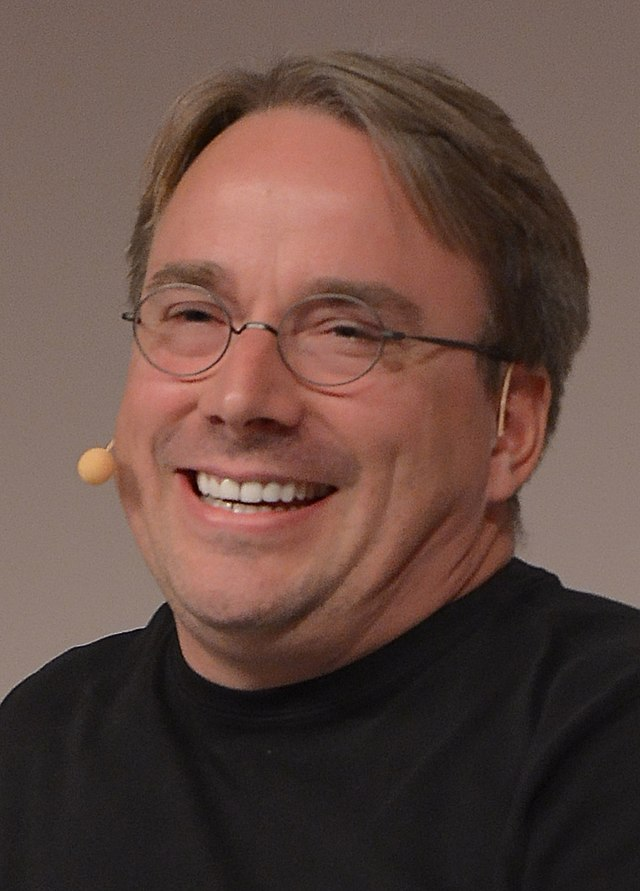
\includegraphics[height=5cm, keepaspectratio]{./resources/Torvalds.jpg}
                    \caption*{Linus B. Torvalds}
                \end{figure}
            }
        \end{column}
    \end{columns}
\end{frame}

\begin{frame}{Verbreitung von Linux}
    Linux gehört heutzutage zu einem der meist verbreitetsten Betriebssysteme überhaupt.

    Einsatzgebiete:
    \begin{itemize}
        \item Android und ChromeOS
        \item Personal Computers
        \item Eingebettete Systeme (Kühlschränke, Router, Medizintechnik, etc.)
        \item Große Teile der Internet Infrastruktur
        % spezifizieren dass es sich bei dem besonders farbigen text um links handelt
        \item Alle der \myhref{https://www.top500.org}{TOP500} Supercomputer
        \begin{itemize}
            \pause
            \item Der SuperMUC (260m vom Hörsaal entfernt) befindet sich auf Platz 31 (Juni 2023)
        \end{itemize}
    \end{itemize}
\end{frame}

\begin{frame}{Was ist Linux}
    Linux ist ein freies (``free'') und ``Open Source'' Betriebssystem. Ein Betriebssystem ist die Schnittstelle zwischen Hardware und Software.

    \vspace{0.3cm}

    Bestandteile eines Betriebssystems (gekürzt):
    \begin{itemize}
        \item Bootloader\textemdash Verantwortlich für den Systemstart
        \item Kernel\textemdash Kern des Betriebssystem (Genaugenommen beschreibt ``Linux'' nur diesen Teil)
        \item Window System\textemdash Ermöglicht graphische Benutzerinterfaces (X, Wayland, etc.)
        \item Desktop Environment\textemdash Interface für den Nutzer (GNOME, KDE, XFCE, etc.)

        % Könnte man ansprechen, geht aber zu weit:
        % Init System
        % Daemons
    \end{itemize}
\end{frame}

% sources:
% - https://robertimschweiler.com/posts/free-software-vs-opensource/
% - https://www.gnu.org/philosophy/free-software-for-freedom.en.html
% - https://www.gnu.org/philosophy/open-source-misses-the-point.html
% - https://www.gnu.org/licenses/license-list.html
% - https://en.wikipedia.org/wiki/Comparison_of_free_and_open-source_software_licenses
\begin{frame}{Free Software vs. Open Source}{Free Software}
    % Mehr kontext von der Person wär nice
    \emph{Free Software} ist von Richard Stallman in 1983 geprägter Begriff.
    % bekannt für GNU ("GNU's Not Unix") und GNU-Linux (das wirklich freie Linux)

    \vspace{0.3cm}

    \emph{Free Software} definiert sich durch 4 Aspekte:
    \begin{itemize}
        \item Freiheit die Software auszuführen
        \item Freiheit die Funktionsweise zu studieren und zu verändern
        \item Freiheit Kopien der Software zu verteilen
        \item Freiheit modifizierte Kopien der Software zu verteilen
    \end{itemize}
    {\Large \MVRightarrow} ``\emph{free}'' ist wie in \emph{free speech} zu sehen nicht wie in \emph{free beer}.

    \vspace{0.3cm}

    Diese Werte werden heute noch von der \myhref{https://www.fsf.org/about}{Free Software Foundation} (\emph{FSF}\,) vertreten durch z.~B. die \myhref{https://opensource.org/license/gpl-3-0}{GNU General Public License}
\end{frame}

\begin{frame}{Free Software vs. Open Source}{Open Source}
    \emph{Open Source} wird von der \myhref{https://opensource.org}{Open Source Initiative} (\emph{OSI}\,) vertreten. Die Werte der \emph{OSI} sind direkt von denen der \emph{FSF} abgeleitet, orientieren sich jedoch ideologisch an den rein praktischen Vorteilen von Quelloffenen Code (Sicherheit, weniger Bugs, etc.).

    \pause
    \vspace{0.3cm}

    \emph{Open Source} ist oft missverständlich. Die Fähigkeit den Source Code anzusehen bedeutet nicht, dass die Software \emph{Free} oder \emph{Open Source} ist!

    \pause
    \vspace{0.3cm}

    % Ich wollte hier eigentlich einen coolen links rechts split machen mit Free Software Lizensen und Open Source Lizensen die nicht auch Free sind, aber look at this (das ist irgendwie stupid): https://en.wikipedia.org/wiki/Comparison_of_free_and_open-source_software_licenses
    % Deswegen jetzt einfach Lizenzen die sowohl FSF als auch OSI approved sind
    Lizenzen die unter \emph{Free Software} und \emph{Open Source} fallen:
    \begin{itemize}
        \item \myhref{https://www.gnu.org/licenses/gpl-3.0.html}{GNU General Public License}
        \item \myhref{https://directory.fsf.org/wiki/License:Apache-2.0}{Apache License}
        \item \myhref{https://directory.fsf.org/wiki/License:BSD-2-Clause-FreeBSD}{FreeBSD License}
        \item \myhref{https://directory.fsf.org/wiki/License:Expat}{Expat License (aka MIT License)}
    \end{itemize}

\end{frame}

\begin{frame}{Linux Distributionen}
    Da Linux nur den Kernel beschreibt und nicht das komplette Betriebssystem gibt es verschiedene Betriebsystem Distributionen (kurz ``Distros''):

    \begin{columns}
        \begin{column}{0.5\textwidth}
            \begin{itemize}
                \item \myhref{https://ubuntu.com}{Ubuntu} (Anfängerfreundlich)
                \begin{itemize}
                    \item \myhref{https://pop.system76.com}{Pop!\_OS}
                \end{itemize}
            
                \item \myhref{https://fedoraproject.org/de}{Fedora} (unsere Empfehlung)
            
                % Arch hat sich der Installationsprozess verbessert
                % Linux from scratch (LFS) ist für eine tiefe lern experience krass (hier startet man nur mim kernel). Ist mehr ein         Buch
                % Gentoo ist mehr wie der alte Arch install
                \item \myhref{https://archlinux.org}{Arch}
                \begin{itemize}
                    \item \myhref{https://manjaro.org}{Manjaro}
                    \item \myhref{https://endeavouros.com}{EndeavourOS}
                \end{itemize}
            \end{itemize}
        \end{column}

        \begin{column}{0.5\textwidth}
            %\begin{figure}[h]
            %    \includegraphics[height=2cm, keepaspectratio]{./resources/Tanenbaum.jpg}
            %    \caption*{Andrew S. Tanenbaum}
            %\end{figure}
            \begin{figure}[h]
                
\includegraphics[width=4cm, keepaspectratio]{./resources/ubuntu.png}
            \end{figure}

            \begin{figure}[h]
                
\includegraphics[width=4cm, keepaspectratio]{./resources/fedora.png}
            \end{figure}
            
            \begin{figure}[h]
                
\includegraphics[width=4cm, keepaspectratio]{./resources/arch.png}
            \end{figure}
        \end{column}
    \end{columns}
\end{frame}

% Die Slide soll Überblick geben über die unterschiede, nicht im tiefsten detail alles erläutern
\begin{frame}{Linux Distributionen}
    Im wesentlichen unterscheiden sich Distributionen in den folgenden Aspekten:
    \begin{itemize}
        \item Umfang und Aktualität der verfügbaren Software
        \item Package Manager
        \item Installer und (Konfigurations-) Tools % ungenau behandeln
        \item Wahl des Desktop Environments % ungenau behandeln
        \item Hardware Unterstützung (z. B. proprietäre Treiber) % ungenau behandeln
        \item Release Cycle (wie oft gibt es neue Versionen\textemdash wie lange werden alte Versionen unterstützt)
        \item Architektur (x86-64 für AMD und Intel, Apple M Prozessoren, etc.) % Apple shift von x86-64 auf M1
        \item Dokumentation % ARCH Wiki namen aufschreiben (allgemein verwendbar).
        \item Support % Ubuntuusers, Stack Exchange namen aufschreiben
        \item Lizenzierung
    \end{itemize}
\end{frame}

\section{Das Filesystem}

% Entwickler der Filesysteme dynamisch per hand hinschreiben (Microsoft, Oracle, etc.)
\begin{frame}{Filesysteme}
    Das Filesystem dient der Organisation von Dateien und Medien auf einem physischen Speichermedium (HDD, SSD, USB-Stick, etc.). Es gibt viele verschiedene Möglichkeiten ein Filesystem aufzusetzen:
    \begin{itemize}
        \pause
        \item Linux typisch:
        \begin{itemize}
            \item ext4
            \item Btrfs
        \end{itemize}

        \pause
        \item Windows typisch:
        \begin{itemize}
            \item FAT32 % bsp wie groß 4gb sind. So typische DVD size, 4GB hinschreiben
            \item exFAT
            \item NTFS
        \end{itemize}

        \pause
        \item MacOS typisch:
        \begin{itemize}
            \item APFS
            \item HFS+
        \end{itemize}
    \end{itemize}
\end{frame}

% Slide drinlassen aber nicht besonders drauf eingehen
% Es reicht zu sagen dass es kompatibilitäts schwierigkeiten gibt
\begin{frame}{Filesysteme}
    Achtung: Nicht jedes Filesystem wird automatisch von jedem Betriebssystem erkannt! Gegebenenfalls müssen züsatzliche Treiber installiert werden.

    \vspace{0.3cm}

    Übersicht:
    \begin{itemize}
        \item NTFS\textemdash Fedora und Ubuntu kommen mit Treibern; MacOS kann Dateien nur lesen
        \item FAT32\textemdash Wird vom Linux Kernel unterstützt; MacOS volle unterstütztung
        \item ext4\textemdash Auf Windows und MacOS nur mit zusätzlichen Treibern möglich
    \end{itemize}
\end{frame}

% Ich bin mir unsicher über das layout der Slide
% Die gemischte nutzung von mintinline und TUMCodeInline ist tatsächlich bewusst
% Vielleicht hier schon auf hidden files eingehen (Unix hidden files mit .)
\begin{frame}{Filesystem Pfade}
    Über Dateipfade kann man u. A.
    \begin{itemize}
        \item leichter durch das Filesystem navigieren
        \item die Ein und Ausgaben von Programmen spezifizieren
    \end{itemize}

    \vspace{0.3cm}

    Pfade sind ``case-sensitive'' (\mintinline{sh}{file} \(\ne\) \mintinline{sh}{File}) und Abschnitte (Ordner) eines Pfades werden durch \mintinline{sh}{/} getrennt.

    \vspace{0.3cm}

    Bei Dateipfaden wird zwischen \emph{Absoluten} und \emph{Relativen} Pfaden unterschieden:
    \begin{itemize}
        % programme sind dateien ist nicht unbedingt klar
        % grep ist eine datei, und dateien können auch programme sein
        \item Absolute Pfade beginnen bei der Dateisystem Root (``\mintinline{sh}{/}''):\\\TUMCodeInline{sh}{/bin/grep}\
        \item Relative Pfade sind relativ zum \emph{CWD} (``current working directory''):\\\TUMCodeInline{sh}{vorkurs/linux.pdf}
    \end{itemize}
\end{frame}

% Changed pwd (meaning "personal working directory", not the command) to cwd (current working directory). Which name to use is honestly kind of confusing and doesn't matter too much in reality. Anyway, cwd is the BSD way which is fine by me, which also avoids confusion with the command pwd ("print working directory").
% https://en.wikipedia.org/wiki/Working_directory
\begin{frame}{Filesystem Pfade}
    \centering
    \begin{tikzpicture}[every node/.style={shape=rectangle, draw, minimum width=4em, minimum height=2em}]
        % === nodes ===

        % root node (green highlight on 2)
        \visible<1,3|handout:0>{\node(root){\mintinline{sh}{/}};}
        \visible<2|handout:1>{\node(root)[draw=TUMGreen, very thick]{\mintinline{sh}{/}};}

        % root -> bin -> grep (green highlight on 2)
        \visible<1,3|handout:0>{\node(root_bin)[below left=1.6em and 30mm of root]{\mintinline{sh}{bin}};}
        \visible<2|handout:1>{\node(root_bin)[below left=1.6em and 30mm of root, draw=TUMGreen, very thick]{\mintinline{sh}{bin}};}
        \visible<1,3|handout:0>{\node(root_bin_grep)[below=1.6em of root_bin]{\mintinline{sh}{grep}};}
        \visible<2|handout:1>{\node(root_bin_grep)[below=1.6em of root_bin, draw=TUMGreen, very thick]{\mintinline{sh}{grep}};}

        % cwd marking on yuuko
        % root -> home -> yuuko -> vorkurs --> linux.pdf (green highlight on 3)
        %                                  --> students.txt
        \node(root_home)[below=1.6em of root]{\mintinline{sh}{home}};
        \node(root_home_yuuko)[below=1.6em of root_home, draw=TUMBlue, very thick]{\mintinline{sh}{yuuko}};
        \node(cwd)[draw=none, minimum width=0, minimum height=0, above right=0 and -1.8em of root_home_yuuko]{\footnotesize \bf\color{TUMBlue}{CWD}};
        \visible<1,2|handout:0>{\node(root_home_yuuko_vorkurs)[below=1.6em of root_home_yuuko]{\mintinline{sh}{vorkurs}};}
        \visible<3|handout:1>{\node(root_home_yuuko_vorkurs)[below=1.6em of root_home_yuuko, draw=TUMOrange, very thick]{\mintinline{sh}{vorkurs}};}
        \visible<1,2|handout:0>{\node(root_home_yuuko_vorkurs_linux)[below left=1.6em and 0 of root_home_yuuko_vorkurs]{\mintinline{sh}{linux.pdf}};}
        \visible<3|handout:1>{\node(root_home_yuuko_vorkurs_linux)[below left=1.6em and 0 of root_home_yuuko_vorkurs, draw=TUMOrange, very thick]{\mintinline{sh}{linux.pdf}};}
        \node(root_home_yuuko_vorkurs_students)[below right=1.6em and 0 of root_home_yuuko_vorkurs]{\mintinline{sh}{students.txt}};

        % root -> usr
        \node(root_usr)[below right=1.6em and 30mm of root]{usr};

        % === lines ===

        % from root
        \visible<1,3|handout:0>{\myline{root}{root_bin}}
        \visible<2|handout:1>{\myline[TUMGreen]{root}{root_bin}}
        \myline{root}{root_home}
        \myline{root}{root_usr}

        % from bin
        \visible<1,3|handout:0>{\myline{root_bin}{root_bin_grep}}
        \visible<2|handout:1>{\myline[TUMGreen]{root_bin}{root_bin_grep}}

        % from home
        \myline{root_home}{root_home_yuuko}

        % from yuuko
        \visible<1,2|handout:0>{\myline{root_home_yuuko}{root_home_yuuko_vorkurs}}
        \visible<3|handout:1>{\myline[TUMOrange]{root_home_yuuko}{root_home_yuuko_vorkurs}}

        % from vorkurs
        \visible<1,2|handout:0>{\myline{root_home_yuuko_vorkurs}{root_home_yuuko_vorkurs_linux}}
        \visible<3|handout:1>{\myline[TUMOrange]{root_home_yuuko_vorkurs}{root_home_yuuko_vorkurs_linux}}
        \myline{root_home_yuuko_vorkurs}{root_home_yuuko_vorkurs_students}

        % === path text ===
        \visible<2|handout:1>{\node[left=3.2em of root, draw=none]{\bf \color{TUMGreen}{\mintinline{sh}{/bin/grep}}};}
        \visible<3|handout:1>{\node[right=3.2em of root_home_yuuko, draw=none]{\bf \color{TUMOrange}{\mintinline{sh}{vorkurs/linux.pdf}}};}
    \end{tikzpicture}
\end{frame}

\begin{frame}{Filesystem Pfade}
    Bedienhilfen (Aktuelles \emph{CWD} ist \TUMCodeInline{sh}{/home/yuuko} für die Beispiele):
    \begin{itemize}
        \item Mit \mintinline{sh}{.} wird das aktuelle Verzeichnis referenziert\\\TUMCodeInline{sh}{./vorkurs/linux.pdf} ist das gleiche wie \TUMCodeInline{sh}{vorkurs/linux.pdf}
        \item Mit \mintinline{sh}{..} wird das Oberverzeichnis referenziert\\\TUMCodeInline{sh}{../yuuko/vorkurs/linux.pdf} ist das gleiche wie \TUMCodeInline{sh}{vorkurs/linux.pdf}
        \item Mit \mintinline{sh}{~} wird das Home-Verzeichnis referenziert (also: \TUMCodeInline{sh}{/home/yuuko})
    \end{itemize}

    \vspace{0.3cm}

    Jeder Nutzer bekommt ein eigenes Home-Verzeichnis \TUMCodeInline{sh}{/home/<username>}.
    \begin{itemize}
        \item Nutzerspezifische Dateien werden diesem Verzeichnis untergeordnet (Konfigurationsdateien, Dokumente, Bilder, usw.)
    \end{itemize}
\end{frame}

\begin{frame}[fragile]{Filesystem Pfade}
    %"Datei- und Ordnernamen" stimmt (https://www.duden.de/sprachwissen/sprachratgeber/Bindestrich-als-Erganzungsstrich)
    % hab von sh auf text gewechselt weil ich die pygments bei ' unschön fand
    % TODO: Lösung finden damit die source files halbwegs konsistent sind
    Datei- und Ordnernamen mit Leerzeichen müssen in Dateipfaden mit \mintinline{text}{"} oder \mintinline{text}{'} umfasst werden:
    \begin{itemize}
        \item \TUMCodeInline{text}{vorkurs/"ordner mit spaces"/datei.txt}
        \item \TUMCodeInline{text}{vorkurs/'ordner mit spaces'/datei.txt}
    \end{itemize}

    \vspace{0.3cm}

    Unterschiede zu anderen Betriebssystemen:
    \begin{itemize}
        \item MacOS basiert wie Linux auf Unix. Dadurch sind die Unterschiede recht gering.
        \item Windows nutzt \mintinline{text}{\} anstelle von \mintinline{text}{/} und der physische Datenträger wird in absoluten Pfaden mit angegeben: \TUMCodeInline{text}{C:\Users\<username>}
    \end{itemize}
\end{frame}

\section{Das Terminal}

\begin{frame}{Was ist das Terminal}
    Das Terminal ist die rudimentärste Form mit einem Computer zu intagieren. Vor richtigen Graphical User Interfaces (GUI) war es oftmals die einzige Möglichkeit mit Computern zu intagieren.

    \vspace{0.3cm}

    Im Terminal werden:
    \begin{itemize}
        \item Kommandos zur Ausführung vom Nutzer eingegeben
        \item Ergebnisse von ausgeführten Kommandos in Textform angezeigt
        \item Über das Terminal kann alles gemacht werden (Systemsteuerung, Office Arbeit, Mail, etc.)
        % Mail ist jetzt kein use case den ich von den Studis erwarten würde, es soll einfach nur illustrieren, dass das Terminal mächtig ist. Unter Office Arbeit zähle ich auch Code editing, compilation, debugging, etc.
    \end{itemize}
\end{frame}

\begin{frame}{Warum sollte man das Terminal benutzen können}
    \begin{itemize}
        \item Interaktion mit dem Computer ist effizient und präzise
        \item Eignet sich gut zur Automatisierung (durch z. B. Scripts)
        \item Flexibilität in der Programmnutzung (verschiedene Programme können sinnvoll interagieren)
        \item Ressourcenarm und universell:
        \begin{itemize}
            \item Remote Verbindungen über ein Terminal benötigen wenig Bandbreite
            \item Remote Verbindungen mit Terminals sind i. d. R. immer möglich
            \item Die nutzung des Terminals ist auf jedem Computer vergleichbar
        \end{itemize}

        \item Viele Server Systeme bieten keine GUI
        \item Viele tools brauchen oder bieten keine GUI
    \end{itemize}
\end{frame}

% https://unix.stackexchange.com/questions/285575/whats-the-difference-between-a-flag-an-option-and-an-argument
\begin{frame}[fragile]{Command Line Arguments}
    \begin{TUMCodeBlock}{Command Arguments and Options}{text}
        command [OPTION...] arguments
    \end{TUMCodeBlock}

    \vspace{0.3cm}

    \begin{itemize}
        \item \TUMCodeInline{text}{command}\textemdash Das auszuführende Kommando

        \item \TUMCodeInline{text}{[OPTION...]}\textemdash Optionen für das Kommando-Verhalten
        \begin{itemize}
            \item Unterscheidung in \emph{Long-Option} (z. B. \TUMCodeInline{text}{--version}) und \emph{Short-Option} (z. B. \TUMCodeInline{text}{-v})
            \item Manche \emph{Options} nehmen auch selbst weitere Argumente
            \item \emph{Options} ohne \emph{arguments} werden auch \emph{Flags} genannt
            \item Nützliche \emph{Flags}: \TUMCodeInline{text}{--help} (bzw. \TUMCodeInline{text}{-h}) und \TUMCodeInline{text}{--version} (bzw. \TUMCodeInline{text}{-v})
        \end{itemize}

        \item \TUMCodeInline{text}{arguments}\textemdash Weitere Argumente (z. B. Dateien, Pfade, etc.)
    \end{itemize}

    \pause
    \vspace{0.3cm}

    \textbf{HINWEIS:} Nicht jedes Command ist konform mit dieser Darstellung.
    % manche programme nehmen anstelle von '-' '/' für z. B. flags (bei gpg oder windows cmd)
\end{frame}

% man, ls, cd, rm, mkdir, touch, cat, sudo, echo
% die reichen für eine basic benutzung der kommandozeile und vermutlich für das erste Aufgabenblatt
\begin{frame}{Essentielle Commands}
    % TAR XKCD
    \begin{figure}[h]
        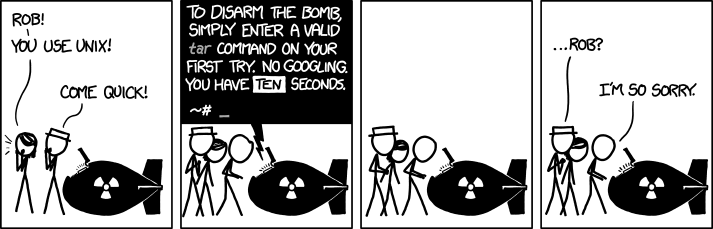
\includegraphics[width=14.5cm, keepaspectratio]{./resources/tar.png}
        \caption*{\myhref{https://xkcd.com/1168/}{xkcd 1168}}
    \end{figure}

    % tar command beispiel, den joke erklären (so doof es auch ist):
    % tar -cvzf archive.tar *

    \pause
    \centering
    Man muss nicht alle Commands auswendig kennen (kann aber praktisch sein)!
\end{frame}

\begin{frame}{Essentielle Commands | \texttt{man}}
    Steht für ``manual''.

    \vspace{0.3cm}

    Ruft die Bedienungsanleitung des angegebenen Objekts auf (z. B. ein Programm).

    \vspace{0.3cm}

    Typische Nutzung:
    \begin{itemize}
        \item \TUMCodeInline{text}{man <command>} (z. B. \TUMCodeInline{sh}{man man})
    \end{itemize}
\end{frame}

\begin{frame}{Essentielle Commands | \texttt{ls}}
    Steht für ``list''.

    \vspace{0.3cm}

    Auflistung des Ordner Inhalts.

    \vspace{0.3cm}

    Typische Nutzung:
    \begin{itemize}
        \item \TUMCodeInline{text}{ls}
        \item \TUMCodeInline{text}{ls path/to/folder}
        \item \TUMCodeInline{text}{ls -a}\textemdash Zeigt auch hidden files (Dateien/Ordner die mit \TUMCodeInline{sh}{.} anfangen) an
        \item \TUMCodeInline{text}{ls -l}\textemdash Zeigt Zusatzinformationen an (Typ, Nutzungsrechte, Größe, Datum)
    \end{itemize}
\end{frame}

\begin{frame}{Essentielle Commands | \texttt{cd}}
    Steht für ``change directory''.

    \vspace{0.3cm}

    Wechsel des \emph{current working directory}.

    \vspace{0.3cm}

    Typische Nutzung:
    \begin{itemize}
        \item \TUMCodeInline{text}{cd path/to/folder}
        \item \TUMCodeInline{text}{cd ..}\textemdash Wechsel in den Parent-Ordner
        \item \TUMCodeInline{text}{cd ~}\textemdash Wechsel zum \emph{Home} Verzeichnis
    \end{itemize}
\end{frame}

\begin{frame}{Essentielle Commands | \texttt{pwd}}
    Steht für ``print working directory''.

    \vspace{0.3cm}

    Zeigt das \emph{current working directory} and.

    \vspace{0.3cm}

    Typische Nutzung:
    \begin{itemize}
        \item \TUMCodeInline{text}{pwd}
    \end{itemize}
\end{frame}

\begin{frame}{Essentielle Commands | \texttt{cat}}
    Steht für ``concatenate files and print''.

    \vspace{0.3cm}

    Gibt Dateien auf der Ausgabe aus.

    \vspace{0.3cm}

    Typische Nutzung:
    \begin{itemize}
        \item \TUMCodeInline{text}{cat test.txt}\textemdash Ausgabe der Datei \TUMCodeInline{text}{test.txt}
        \item \TUMCodeInline{text}{cat one.txt two.txt}\textemdash Gibt die dateien \TUMCodeInline{text}{one.txt} und \TUMCodeInline{text}{two.txt} aus
    \end{itemize}
\end{frame}

\begin{frame}{Essentielle Commands | \texttt{echo}}
    Gibt den Angegebenen Text wieder aus.

    \vspace{0.3cm}

    Typische Nutzung:
    \begin{itemize}
        \item \TUMCodeInline{text}{echo "beliebiger Text"}
    \end{itemize}
\end{frame}

\begin{frame}{Essentielle Commands | \texttt{mkdir}}
    Steht für ``make directory''.

    \vspace{0.3cm}

    Erstellt Ordner.

    \vspace{0.3cm}

    Typische Nutzung:
    \begin{itemize}
        \item \TUMCodeInline{text}{mkdir folder}\textemdash Erstellt den Ordner \TUMCodeInline{text}{folder} im aktuellen \emph{CWD}
        \item \TUMCodeInline{text}{mkdir f1 f2 f3}\textemdash Erstellt die Ordner \TUMCodeInline{text}{f1}, \TUMCodeInline{text}{f2} und \TUMCodeInline{text}{f3} im aktuellen \emph{CWD}
    \end{itemize}
\end{frame}

\begin{frame}{Essentielle Commands | \texttt{rm}}
    Steht für ``remove''.

    \vspace{0.3cm}

    Löscht Ordner und Dateien.

    \vspace{0.3cm}

    Typische Nutzung:
    \begin{itemize}
        \item \TUMCodeInline{text}{rm test.txt}
        \item \TUMCodeInline{text}{rm -d empty-folder}
        \item \TUMCodeInline{text}{rm -r nonempty-folder}\textemdash Ordner mit Inhalt müssen ``rekursiv'' gelöscht werden {\Large \MVRightarrow} Der Inhalt des Ordners wird nun explizit gelöscht
        \item \TUMCodeInline{text}{rm -f test.txt}\textemdash Erzwingt sofortige Löschung und ignoriert nicht existente Dateien
    \end{itemize}
\end{frame}

\begin{frame}{Essentielle Commands | \texttt{touch}}
    Änderung der Zeitstempel einer Datei oder eines Ordners.

    \vspace{0.3cm}

    Typische Nutzung:
    \begin{itemize}
        \item \TUMCodeInline{text}{touch test.txt}\textemdash Aktualisiert den Zeitstempel der Datei \TUMCodeInline{sh}{test.txt} oder erstellt eine neue leere Datei mit diesem Namen falls diese nicht existiert
    \end{itemize}
\end{frame}

\begin{frame}{Essentielle Commands | \texttt{mv}}
    Steht für ``move''.

    \vspace{0.3cm}

    Verschiebung oder Umbenennung von Dateien.

    \vspace{0.3cm}

    Typische Nutzung:
    \begin{itemize}
        \item \TUMCodeInline{text}{mv path/to/file new/path/}\textemdash Verschiebt \TUMCodeInline{text}{file} von \TUMCodeInline{text}{path/to/} nach \TUMCodeInline{text}{new/path/}
        \item \TUMCodeInline{text}{mv path/to/file new/path/elif}\textemdash Wie oben, die Datei wird zusätzlich von \TUMCodeInline{text}{file} zu \TUMCodeInline{text}{elif} umbenannt
    \end{itemize}
\end{frame}

\begin{frame}{Essentielle Commands | \texttt{cp}}
    Steht für ``copy''.

    \vspace{0.3cm}

    Kopieren von Dateien und Ordnern.

    \vspace{0.3cm}

    Typische Nutzung:
    \begin{itemize}
        \item \TUMCodeInline{text}{cp path/to/file other-path/to/copy}\textemdash Kopiert \TUMCodeInline{text}{file} von \TUMCodeInline{text}{path/to/} nach \TUMCodeInline{text}{other-path/to/} und speichert die Kopie als \TUMCodeInline{text}{copy}
    \end{itemize}
\end{frame}

% https://www.techtarget.com/searchsecurity/definition/sudo-superuser-do
\begin{frame}{Essentielle Commands | \texttt{sudo}}
    Steht für ``su-do'' (``substitute user do'', veraltet auch ``superuser do'').

    \vspace{0.3cm}

    Erlaubt das Ausführen eines Commands mit den Rechten eines anderen Nutzers (meistens mit denen des \emph{superuser's}).

    \vspace{0.3cm}

    \TUMCodeInline{text}{sudo} wird oft benötigt wenn ein Command nicht mit den Nutzerrechten ausgeführt werden kann:
    \begin{itemize}
        \item \TUMCodeInline{text}{sudo dnf install terminator}\textemdash Die Installation von Packages (hier ``terminator'' ein Terminal emulator) erfordert die Berechtigung des \emph{superuser's}
    \end{itemize}
\end{frame}

% https://www.w3resource.com/linux-system-administration/control-operators.php
\begin{frame}[fragile]{Control Operators}
    \TUMCodeInline{text}{&&}
    \begin{itemize}
        \item Konkatenation von 2 Commands. Letzteres wird nur ausgeführt wenn das erste \textbf{erfolgreich} war.
        \item Bsp.: \TUMCodeInline{text}{cd MaybeExists && ls}
    \end{itemize}

    \vspace{0.3cm}

    \TUMCodeInline{text}{||}
    \begin{itemize}
        \item Konkatenation von 2 Commands. Letzteres wird nur ausgeführt wenn das erste \textbf{fehlgeschlagen} ist.
        \item Bsp.: \TUMCodeInline{text}{cd MaybeExists || echo "Folder does not exist!"}
    \end{itemize}

    \vspace{0.3cm}

    \TUMCodeInline{text}{;}
    \begin{itemize}
        \item Konkatenation mehrerer Commands.
        \item Bsp.: \TUMCodeInline{text}{echo "Hello"; echo "World"; echo "!"}
    \end{itemize}
\end{frame}

\begin{frame}{Control Operators}
    \TUMCodeInline{text}{&}
    \begin{itemize}
        \item Das vorangegangen Command wird im Hintergrund ausgeführt.
        \item Bsp.: \TUMCodeInline{text}{sleep 10 &}
    \end{itemize}

    \vspace{0.3cm}

    \TUMCodeInline{text}{>} und \TUMCodeInline{text}{>>}
    \begin{itemize}
        \item Umleitung der Ausgabe in eine Datei. \TUMCodeInline{text}{>} löscht die Datei davor.
        \item Bsp.: \TUMCodeInline{text}{echo "HelloWorld!" > greeting.txt} bzw. \TUMCodeInline{text}{echo "HelloWorld!" >> greeting.txt}
    \end{itemize}

    \vspace{0.3cm}

    \TUMCodeInline{text}{|} (genannt ``Pipe'')
    \begin{itemize}
        \item Die Ausgabe des vorangegangeng Commands ist die Eingabe des folgenden Commands.
        % zuerst einmal fortune ausführen und dann einmal cowsay
        \item Bsp.: \TUMCodeInline{text}{fortune | cowsay}
    \end{itemize}
\end{frame}

\begin{frame}[fragile]{Control Operators}
    \begin{TUMCodeBlock}{Beispiel Terminal Fenster}{sh}
        yuuko@kyoto:~/Vorkurs$ ls
        Folien  students.txt
        yuuko@kyoto:~/Vorkurs$ fortune | cowsay
         _____________________________
        < Avoid reality at all costs. >
         -----------------------------
                \   ^__^
                 \  (oo)\_______
                    (__)\       )\/\
                        ||----w |
                        ||     ||
    \end{TUMCodeBlock}
\end{frame}

\begin{frame}{Tipps und Tricks}
    Bedienhilfen:
    \begin{itemize}
        \item Aufruf voheriger Befehle durch ``Pfeiltaste nach oben''
        \item Angefangene Pfade können oft mit \emph{Tab} vervollständigt werden
        \item Löschen der aktuellen Eingabe mit \emph{Strg+U}
        \item Abbrechen eines laufenden Befehls mit \emph{Strg+C}
        \item Kopieren aus dem Terminal mit \emph{Strg+Shift+C}
        \item Kopieren in das Terminal mit \emph{Strg+Shift+V}
        \item Löschen des Bildschirmtexts mit \emph{Strg+L} (Terminal History bleibt bestehen)
        \item Löschen des Bildschirmtexts mit dem Command \TUMCodeInline{text}{clear} (Terminal History wird gelöscht)
    \end{itemize}
\end{frame}

% This marks the end of the first lecture
\mode<handout:0>{\section{Pause}} % not included on handout

\section{Package Management}

\begin{frame}{Package Management}
    Package Manager verwalten die Software die auf einem System installiert ist. Zur Verwaltung gehören u. A.:
    \begin{itemize}
        \item Installation
        \item Aktualisierung
        \item Deinstallation
        % bsp.: 1) sudo dnf install terminator
        %       2) sudo dnf remove terminator
        \item Überprüfung von Software Dependencies
    \end{itemize}

    \pause
    \vspace{0.3cm}

    Durch Package Manager wird die Installation von Software erleichtert:
    \begin{itemize}
        \item Jegliche Software wird über die gleiche Methode installiert
        \item Konflikte zwischen Software Paketen werden erkannt und u. U. verhindert
        \item Keine seperaten Installer Programme die:
        \begin{itemize}
            \item Zusatzsoftware installieren und Werbung zeigen
            \item über nicht vertrauenswürdige Webseiten herunterzuladen sind
        \end{itemize}
    \end{itemize}
\end{frame}

\begin{frame}{Package Management}
    Package Manager greifen für die Installation von Software auf spezielle Software Pakete zurück die sich in sog. Repositories befinden.

    \vspace{0.3cm}

    Linux Distribution kommen mit einem Package Manager dessen Software Repositories von den jeweiligen Entwicklern instand gehalten wird.
    \begin{itemize}
        \item Ubuntu: \myhref{https://ubuntu.com/server/docs/package-management}{apt}
        \item Fedora: \myhref{https://docs.fedoraproject.org/en-US/quick-docs/dnf}{dnf}
        \item Arch: \myhref{https://wiki.archlinux.org/title/pacman}{pacman}
        \item OpenSUSE: \myhref{https://documentation.suse.com/smart/systems-management/html/concept-zypper/index.html}{Zypper}
        \item Und viele mehr! (xbps, eopkg, yum, \dots)
        % Vielleicht noch mehr nennen um die insane Menge besser darzustellen
        % Hab das jetzt mal relativ lazy hinzugefügt. Feel free to suggest something else.
        % Hauptsächlich weil mir xbps und eopkg nicht viel sagt
    \end{itemize}
\end{frame}

\begin{frame}{Package Management}
    Unter Linux gibt es auch Distributionsübergreifende Package Manager die zusätzlich installiert werden können:
    \begin{itemize}
        \item \myhref{https://snapcraft.io/about}{Snap}
        \item \myhref{https://flatpak.org/}{Flatpak}
        \item \myhref{https://docs.brew.sh/Homebrew-on-Linux}{Homebrew}
        \item \myhref{https://nixos.org}{Nix}
    \end{itemize}

    \vspace{0.3cm}

    Vorteile von zusätzlichen Package Managern:
    \begin{itemize}
        \item Installation von Software die nicht in den Repositories des ``Host'' Package Managers vorliegen
        \item U. U. aktuellere Software Versionen
        \item Package Manager spezifische vorteile (z. B. Cross-Platform)
        % in den Klammern vielleicht noch mehr nennen
    \end{itemize}
\end{frame}

\begin{frame}{Package Management}
    Package Manager können auch unter Windows und MacOS genutzt werden.

    \vspace{0.3cm}

    Windows:
    \begin{itemize}
        \item \myhref{https://learn.microsoft.com/de-de/windows/package-manager/winget}{winget} (Offiziell von Microsoft)
        \item \myhref{https://scoop.sh}{scoop}
        \item \myhref{https://chocolatey.org}{chocolatey}
        % TODO es gibt tatsächlich noch paar mehr, kann man sich überlegen die hier hinzuzufügen
    \end{itemize}

    \vspace{0.3cm}

    MacOS:
    \begin{itemize}
        \item \myhref{https://brew.sh}{Homebrew}
        \item \myhref{https://www.macports.org}{MacPorts}
        \item \myhref{https://nixos.org}{Nix}
    \end{itemize}
\end{frame}

\section{Access Control}

\begin{frame}{Access Control\textemdash Generelle Konzepte}
    Verwaltung von Nutzungsrechten ist wichtig aber auch schwierig:
    \begin{itemize}
        \item Dateien unterliegen oft einem ``Geheimhaltungsgrad'' (privates, Krankenakte, Klausuren, etc.)
        \item Oft interagieren viele Leute mit dem gleichen System (Unternehmen, Krankenhäuser, Universitäten, etc.)
    \end{itemize}

    \pause
    \vspace{0.3cm}

    Es gibt viele Modelle um eine Access Control zu realisieren:
    \begin{itemize}
        \item Discretianoray Access Control (\emph{DAC}\,)
        \item Role-based Access Control (\emph{RBAC}\,)
        \item Mandatory Access Control (\emph{MAC}\,)
        \item Bell-LaPadula Modell (\emph{BLP}\,)
        \item Zugriffsmatrix Modell (\emph{ZM}\,)
    \end{itemize}
    {\Large \MVRightarrow} Diese Modelle werden Sie im Fach \emph{IT-Sicherheit} noch genauer besprechen.
\end{frame}

% Folgende Optionen werden nicht angesprochen: Recursive, Preserve-Root, Reference-File, Setuid, Setgid, Sticky Bit
% Ich denke, dass das den Rahmen sprengt
\begin{frame}[fragile]{Access Control\textemdash Linux}
    Unix (bzw. Linux) nutzt eine Variante des Zugriffsmatrix Modells: \emph{Access-Control-List} (\emph{ACL}\,)
    \begin{itemize}
        \item \emph{ACL} ist aus Objekt-Sicht {\Large \MVRightarrow} Jedes Datum beinhaltet die eigenen Rechte
        \item Rechtevergabe eines Datums an \emph{Owner}, \emph{Group} und \emph{Other}
        \item Rechte beinhalten:
        \begin{itemize}
            \item \textbf{R}ead (Bei Ordnern kann damit der Inhalt gelistet werden)
            \item \textbf{W}rite
            \item e\textbf{X}ecute (Bei Ordnern wird die traversierung erlaubt)
        \end{itemize}
    \end{itemize}

    \pause
    \vspace{0.3cm}

    \begin{TUMCodeBlock}{}{text}
        drwxr-xr-x 2 mlutt tutors   60160 Sep 17 14:09 Vorlesung
        -rw-r----- 1 mlutt tutors    4096 Sep 14 13:37 Solution-1.pdf
        -rw-r--r-- 1 mlutt students  2048 Sep 13 14:09 Task-1.pdf
    \end{TUMCodeBlock}
\end{frame}

\section{Environment Variables}

\begin{frame}{Environment Variables}
    \emph{Environment Variables} ermöglichen die weitergabe von konfigurierbaren Variablen an Prozesse über deren ``Umgebung''. Diese Variablen enthalten oft Pfade zu Programmen/Daten oder andere Einstellungen.

    \vspace{0.3cm}

    Beispiele für \emph{Environment Variables}:
    \begin{itemize}
        \item HOSTTYPE\textemdash Architektur des Computers (z. B. \emph{x86-64})
        \item HOME\textemdash Pfad zu \TUMCodeInline{sh}{/home/<username>}
        \item PWD\textemdash Pfad zum aktuellen ``working directory''
        \item PATH\textemdash Pfade zu ausführbaren Programmen
        \item TEMP/TMP\textemdash Ablageort für Temporäre Dateien
    \end{itemize}

    % Nicht wirklich necessary, kann man einfach sagen
    %\vspace{0.3cm}
    %Alle Prozesse auf einem Unixoidem Betriebssystem oder Windows erhalten einen eigenen separaten Satz an \emph{Environment Variables} die bei der Erstellung des Prozesses erstellt werden.
\end{frame}

\section{SSH}

%https://wiki.ito.cit.tum.de/bin/view/Informatik/Helpdesk/Ssh/#H1.1.SSHVerbindungmitPasswort
\begin{frame}[fragile]{SSH}
    SSH steht für \emph{Secure Shell}:
    \begin{itemize}
        \item Ermöglicht eine sichere Verbindung zwischen Rechnern in ungesicherten Netzwerken (z. B. Internet)
        \item Dient der sicheren (remote) Systemverwaltung
        \item Identitäten, Passwörter und Daten werden verschlüsselt
    \end{itemize}

    \pause
    \vspace{0.3cm}

    Sie können sich über den SSH Befehl mit der Rechnerhalle verbinden (Authentifizierung über Ihr Passwort):

    \vspace{0.3cm}

    \begin{TUMCodeBlock}{}{sh}
        ssh <username>@lxhalle.in.tum.de
    \end{TUMCodeBlock}
    {\Large \MVRightarrow} Verbindung kann mit \TUMCodeInline{text}{exit} beendet werden.

    \vspace{0.3cm}

    % Needed to escape # in URL
    Bei der ersten Verbindung sollte man die \myhref{https://wiki.ito.cit.tum.de/bin/view/Informatik/Helpdesk/Ssh/\#H0.Fingerprints}{Fingerprints} der Rechnerhalle verifizieren.
\end{frame}

% https://www.bsi.bund.de/SharedDocs/Downloads/EN/BSI/Publications/TechGuidelines/TG02102/BSI-TR-02102-1.pdf?__blob=publicationFile
% Federal Office for Information Security (as of Jan 2023)
\begin{frame}{SSH Keys}
    Eine authentifizierte Verbindung geht auch ohne die eingabe des Passworts über SSH Schlüsselpaare. \myhref{https://wiki.ito.cit.tum.de/bin/view/Informatik/Helpdesk/Ssh/\#H1.3.SSHKey}{Generierung}:
    \begin{itemize}
        % Increased bit depth for RSA Key for compliance with current standards
        \item \TUMCodeInline{sh}{ssh-keygen -t rsa -b 4096} für ein \emph{RSA} (Rivest-Shamir-Adleman) Schlüsselpaar
        \item \TUMCodeInline{sh}{ssh-keygen -t ed25519} für ein \emph{ECC} (Elliptic Curve Cryptography) Schlüsselpaar
    \end{itemize}

    \vspace{0.3cm}

    Ein Schlüsselpaar besteht aus einem:
    \begin{itemize}
        \item öffentlichen Schlüssel (z. B. \TUMCodeInline{sh}{~/.shh/id_ed25519.pub})
        \item privaten Schlüssel (z. B. \TUMCodeInline{sh}{~/.ssh/id_ed25519})
    \end{itemize}
    {\Large \MVRightarrow} Man spricht hier auch von \emph{asymmetrischen Schlüsseln}!

    \vspace{0.3cm}

    \begin{itemize}
        % Hier erwähnen, dass in den späteren vcs Slides noch genauer darauf eingegangen wird
        \item Der öffentliche Schlüssel darf an Services weitergegeben werden (\myhref{https://wiki.ito.cit.tum.de/bin/view/Informatik/Helpdesk/Ssh}{Rechnerhalle}, \myhref{https://doku.lrz.de/ssh-tutorial-10746941.html}{LRZ}, \myhref{https://docs.github.com/en/authentication/connecting-to-github-with-ssh}{GitHub}, etc.)
        \item Der private Schlüssel darf \emph{niemals} preisgegeben werden!
    \end{itemize}
\end{frame}

% Hier muss man vorsichtig sein. Die eigentliche SSH Verbindung ist symmetrisch verschlüsselt (AES). Aufpassen, dass durch die Folien nicht etwas falsches suggeriert wird. Eine Sinnvolle Waage finden zwischen dem was im Vorkurs für ein basic Verständnis wichtig ist und dem was in der Realität passiert. Anwendungsbezug prüfen und im Zweifel den "Content Scope" reduzieren.
%\begin{frame}{Asymmetrische Verschlüsselung}
    % Ich glaub ich yeete diese Slide. Sie ist nicht strictly necessary
%\end{frame}

\section{Code Editing}

\begin{frame}{Editors}
    % TAR XKCD
    \begin{figure}[h]
        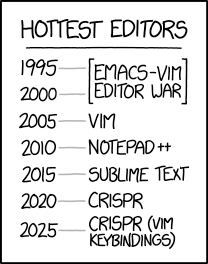
\includegraphics[width=4.5cm, keepaspectratio]{./resources/hottest_editors.png}
        \caption*{\myhref{https://xkcd.com/1823/}{xkcd 1823}}
    \end{figure}

    % auch hier den joke wieder ein bissel erklären (ist doof, aber eh...)
    % Letztendendes will ich mit dem xkcd sagen, dass die Unterscheidung Text Editor und Code Editor beschissen ist.
    % Im Internet findet man dazu nur wild unterschiedliche Definitionen die nicht miteinander kompatibel sind.
    % Der xkcd fasst das super zusammen weil dieser 'Editoren' noch allgemeiner sieht. Weswegen 'crispr' gelistet wird (GEN-Editor)
\end{frame}

\begin{frame}{Text Editors und IDE's}
    \emph{Text Editoren} sind leichtgewichtige Programme die primär zur Text bearbeitung dienen, aber auf die Nutzung mit Code angepasst werden können:
    \begin{itemize}
        \item nano
        \item vi, \myhref{https://www.vim.org/}{vim}, \myhref{https://neovim.io}{neovim}
        \item \myhref{https://www.sublimetext.com}{Sublime Text}
        \item \myhref{https://code.visualstudio.com}{Visual Studio Code}
        % "freiere" Version von VS Code ohne Telemetrie von Microsoft
        \item \myhref{https://vscodium.com}{VSCodium}
    \end{itemize}

    \pause
    \vspace{0.3cm}

    \emph{IDE} steht für \emph{Integrated Development Environment}. \emph{IDE's} bündeln noch zusätzliche Tools die bei der Erstellung von Code helfen:
    \begin{itemize}
        \item \myhref{https://www.jetbrains.com/de-de/idea}{IntelliJ}
        \item \myhref{https://www.eclipse.org/downloads}{Eclipse}
        \item \myhref{https://visualstudio.microsoft.com/de}{Visual Studio}
    \end{itemize}
\end{frame}

\begin{frame}{Terminal Editoren}
    % immer available
    Terminal Editoren wie \emph{nano}, \emph{vi}, \emph{vim} sind fast überall vorinstalliert.

    \pause
    \vspace{0.3cm}

    \textbf{nano}:
    \begin{itemize}
        \item Einfach in der Bedienung
        \item In der Kurzanleitung von \emph{nano} ist mit \TUMCodeInline{text}{^} die Taste \emph{Strg} gemeint
        \item Mit \TUMCodeInline{text}{^X} (\emph{Strg+X}\,) wird \emph{nano} beendet
        \item Mit \TUMCodeInline{text}{^O} (\emph{Strg+O}\,) wird der modifizierte Inhalt gespeichert 
    \end{itemize}
\end{frame}

\begin{frame}{Terminal Editoren}
    % vi zu vim. in vi keine text objects und konfiguration ist non existent. es gibt nur vanilla insert und normal mode
    % vim hat text object systeme, autocomplete, vimscript, packages plugins, searches, mehr settings wie incremental search, extended normal mode
    % neovim kann lua weil vimscript shit ist, nativer lsp, vim api in lua übersetzt

    \textbf{vim}:
    \begin{itemize}
        \item Arbeitet mit ``Modes'' (wir betrachten nur \textbf{INSERT-MODE} und \textbf{NORMAL-MODE})
        \item \emph{vim} startet im \textbf{NORMAL-MODE}, dieser Modus erlaubt die Nutzung von Editor-Commands:
            \begin{itemize}
                \item \TUMCodeInline{text}{:q}\textemdash ``Quit'' (beendet vim)
                \item \TUMCodeInline{text}{:w}\textemdash ``Write'' (speichert den editierten text)
                \item \TUMCodeInline{text}{:wq}\textemdash ``Write and Quit''
                \item durch anhängen von \TUMCodeInline{text}{!} wird das Command erzwungen
                \item mit \TUMCodeInline{text}{i} wird zum \textbf{INSERT-MODE} gewechselt
            \end{itemize}
        \item Im \textbf{INSERT-MODE} kann der text bearbeitet werden
            \begin{itemize}
                \item mit \emph{ESC} wird zum \textbf{NORMAL-MODE} gewechselt
            \end{itemize}
    \end{itemize}
\end{frame}

\section{Nützliche Commands}
% hier ist dann der ganze rest der commands (htop, grep, less, etc.)
% Die Slides über die commands kann man rauskopieren und dann in ein cheatsheet packen

\begin{frame}{Nützliche Commands | \texttt{grep}}
    Steht für ``\textbf{g}lobal \textbf{r}egular \textbf{e}xpression search and \textbf{p}rint''.

    \vspace{0.3cm}

    Mithilfe von \texttt{grep} können Muster in Dateien gesucht werden. Diese Suche wird durch \emph{RegEx} (Regular Expressions) ermöglicht ({\Large \MVRightarrow} Mehr dazu in der Vorlesung ``Theoretische~Informatik'').

    \vspace{0.3cm}

    % 1973 veröffentlicht und Entwickelt von Ken Thompson
    % Ken nutzte das Programm bereits privat
    % Sein Abteilungsleiter Doug McIlroy (wusste noch nichts von grep) schlug Thompson ein solches Programm vor!
    % Thompson sagte dass er in der Nacht drüber nachdenken wird (nutzte die Zeit aber um Bugs zu fixen und letzte Verbesserungen zu machen) --> Daher auch die misconception, dass grep in einer Nacht geschrieben wurde.

    Typische Nutzung:
    \begin{itemize}
        \item Generell: \TUMCodeInline{text}{grep "RegEx" Datei-Muster}
        \item \TUMCodeInline{text}{grep "test" *.txt}\textemdash Gibt die Zeilen der Eingabedateien (mit Endung \TUMCodeInline{text}{.txt}) die das Muster \emph{test} enthalten aus
        \item \TUMCodeInline{text}{cat *.txt | grep "test"}\textemdash Häufig auch mit Pipes \TUMCodeInline{text}{|} zusammen
        \item Nützliche Optionen sind \TUMCodeInline{text}{-c} (für ``count'') und \TUMCodeInline{text}{-i} {für ``ignore-case''}
    \end{itemize}

    % Options wie -c (count) und -i (ignore-case)

    \vspace{0.3cm}

    \texttt{ripgrep} (Command: \TUMCodeInline{text}{rg}) ist eine alternative Implementation in \myhref{https://www.rust-lang.org}{Rust} ähnlich zu \texttt{grep}.
\end{frame}

\begin{frame}{Nützliche Commands | \texttt{wc}}
    Steht für ``word count''.

    \vspace{0.3cm}
    
    Gibt die Anzahl der in einer Datei enthaltenen Zeilen, Wörter und Bytes aus.

    \vspace{0.3cm}

    Typische Nutzung:
    \begin{itemize}
        \item \TUMCodeInline{text}{wc test.txt}
    \end{itemize}
\end{frame}

\begin{frame}{Nützliche Commands | \texttt{ping}}
    Sendet eine \emph{ICMP ECHO\_REQUEST} an die Angegebene \emph{IP-Adresse} oder \emph{URL} ({\Large \MVRightarrow} Mehr dazu in der Vorlesung ``Grundlagen~Rechnernetze'').

    \vspace{0.3cm}

    Nützlich um die Verfügbarkeit eines Services oder Rechners über das Netzwerk zu überprüfen.

    \vspace{0.3cm}

    Typische Nutzung:
    \begin{itemize}
        \item \TUMCodeInline{text}{ping zulip.in.tum.de}
    \end{itemize}
\end{frame}

\begin{frame}{Nützliche Commands | \texttt{scp}}
    Steht für ``\emph{OpenSSH} secure file copy''

    \vspace{0.3cm}

    Kopieren von Dateien zwischen zwei Rechnern über ein Netzwerk.

    \vspace{0.3cm}

    Typische Nutzung:
    \begin{itemize}
        \item \TUMCodeInline{text}{scp path/to/local/file <username>@<remote-URL>:path/to/remote/copy}
        \item z.B. \TUMCodeInline{text}{scp test.txt <username>@lxhalle.in.tum.de:~/}
    \end{itemize}
\end{frame}

\begin{frame}{Nützliche Commands | \texttt{htop}}
    ``Task Manager'' von Linux.

    \vspace{0.3cm}

    Typische Nutzung:
    \begin{itemize}
        \item \TUMCodeInline{text}{htop}
    \end{itemize}
\end{frame}

\begin{frame}{Nützliche Commands | \texttt{neofetch}}
    Zeigt System-Informationen an.

    \vspace{0.3cm}

    Typische Nutzung:
    \begin{itemize}
        \item \TUMCodeInline{text}{neofetch}
    \end{itemize}
\end{frame}

\begin{frame}{Nützliche Commands | \texttt{more}}
    Der Inhalt langer Dateien oder Output von einem Command wird ``Seitenweise'' angezeigt.

    \vspace{0.3cm}

    Typische Nutzung:
    \begin{itemize}
        \item \TUMCodeInline{text}{cat huge-file | more}
        \item \TUMCodeInline{text}{more huge-file}
    \end{itemize}
\end{frame}

\begin{frame}{Nützliche Commands | \texttt{less}}
    \texttt{less} ist ähnlich zu \texttt{more}, kann aber wesentlich mehr!
    \begin{itemize}
        \item \texttt{less} muss nicht die gesamte Datei eingelesen haben {\Large \MVRightarrow} startet schneller
        \item Durch die Datei kann Zeilenweise gescrollt werden
        \item etc.
    \end{itemize}

    \vspace{0.3cm}

    Typische Nutzung:
    \begin{itemize}
        \item \TUMCodeInline{text}{cat huge-file | less}
        \item \TUMCodeInline{text}{less huge-file}
    \end{itemize}
\end{frame}

\begin{frame}{Nützliche Commands | \texttt{alias}}
    Erstellt ein Alias für ein Nutzerdefiniertes command.

    \vspace{0.3cm}

    Beispiel:
    \begin{itemize}
        \item \TUMCodeInline{text}{alias wisdom="fortune | cowsay"}\textemdash Nun kann \TUMCodeInline{text}{wisdom} anstelle von \TUMCodeInline{text}{fortune | cowsay} benutzt werden
    \end{itemize}

    \vspace{0.3cm}
    Ein Nutzerdefiniertes Alias bleibt nur für eine Session bestehen!
    {\Large \MVRightarrow} Ein persistentes Alias kann mithilfe von Shell-Konfigurationsdateien erstellt werden (z.B. \TUMCodeInline{text}{~/.bashrc} oder \TUMCodeInline{text}{~/.zshrc})
\end{frame}

\begin{frame}{Nützliche Commands | \texttt{history}}
    Zeigt die vorhande history and eingegebenen commands an.

    \vspace{0.3cm}

    Typische Nutzung:
    \begin{itemize}
        \item \TUMCodeInline{text}{history}
    \end{itemize}
\end{frame}

\begin{frame}{Nützliche Commands | \texttt{tree}}
    Zeigt den Filesystembaum ausgehend vom \emph{CWD} an.

    \vspace{0.3cm}

    Typische Nutzung:
    \begin{itemize}
        \item \TUMCodeInline{text}{tree}
    \end{itemize}
\end{frame}

\begin{frame}{Nützliche Commands | \texttt{pushd} und \texttt{popd}}
    Steht für ``push directory'' und ``pop directory''.

    \vspace{0.3cm}

    Erleichtern die Navigation durch die Möglichkeit Dateipfade zwischenzuspeichern.

    \vspace{0.3cm}

    Typische Nutzung:
    \begin{enumerate}
        \item \TUMCodeInline{text}{pushd /bin}\textemdash Speichert das \emph{CWD} und wechselt zu dem Ordner \TUMCodeInline{text}{/bin}
        \item \TUMCodeInline{text}{popd}\textemdash Ändert das aktuelle \emph{CWD} zu dem vorher gespeichertem
    \end{enumerate}
\end{frame}

\end{document}
